\begin{frame}
	\myheading{Module 13.6 : Optimization over images}
\end{frame}

%%%%%%%%%%%%%%%%%%%%%%%%%%%%%%%%%%%%%%%%%%%%%%%%%%%%%%%%%%%%%%%%%%%%%%%%%%%%%%

\begin{frame}
	\begin{columns}
		\column{0.5\textwidth}
		\begin{overlayarea}{\textwidth}{\textheight}
			\input{modules/Module6/tikz_images/input3.tex}
		\end{overlayarea}
		\column{0.5\textwidth}
		\begin{overlayarea}{\textwidth}{\textheight}
			
			\begin{itemize}
				\justifying
				\item<1-> Suppose we want to create an image which looks like a dumbell (or an ostrich, or a car, or just anything)
				\item<2-> In other words we want to create an image such that if we pass it through a trained ConvNet
				it should maximize the probability of the class dumbell
				\item<3-> We could pose this as an optimization problem w.r.t $I\ (i_0,\ i_1,\ \dots,\ i_{mn})$ 
				\onslide<4->{
					\begin{align*}
						\arg       & \max_{I}(S_c(I) - \lambda \Omega(I))         \\
						S_c(I)=       & \text{ Score for class C before softmax}     \\
						\Omega(I)= & \text{ Some regularizer to ensure that  } \\
						           & \text{$I$ looks like an image}                   
					\end{align*}}
							
			\end{itemize}
		\end{overlayarea}
	\end{columns}
\end{frame}

%%%%%%%%%%%%%%%%%%%%%%%%%%%%%%%%%%%%%%%%%%%%%%%%%%%%%%%%%%%%%%%%%%%%%%%%%%%%%%

\begin{frame}
	\begin{columns}
		\column{0.5\textwidth}
		\begin{overlayarea}{\textwidth}{\textheight}
			\input{modules/Module6/tikz_images/input3.tex}
		\end{overlayarea}
		\column{0.5\textwidth}
		\begin{overlayarea}{\textwidth}{\textheight}
			\begin{itemize}
				\justifying
				\item<1-> We can essentially think of the image as a collection of parameters
				\item<2->Keep the weights of trained convolutional neural network fixed
				\item<3->Now adjust these parameters(image pixels) so that the score of a class is maximized
				\item<4->Let us see how
			\end{itemize}
		\end{overlayarea}
				
		
	\end{columns}
\end{frame}

%%%%%%%%%%%%%%%%%%%%%%%%%%%%%%%%%%%%%%%%%%%%%%%%%%%%%%%%%%%%%%%%%%%%%%%%%%%%%%

\begin{frame}
	\begin{overlayarea}{\textwidth}{\textheight}
		\begin{center}
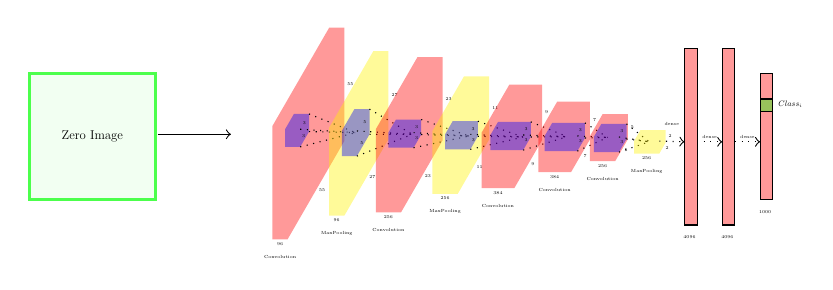
\begin{tikzpicture}[scale=0.32,transform shape]

\pgfsetxvec{\pgfpoint{1cm}{0cm}}
\pgfsetyvec{\pgfpoint{0cm}{1cm}}
\pgfsetzvec{\pgfpoint{-.5cm}{-.866cm}}

\def\cuboid#1#2#3#4#5{
\begin{scope}
\edef\mycolor{#2}
\edef\depth{#3}
\edef\height{#4}
\edef\width{#5}
\draw[black,fill=\mycolor, fill opacity=0.4, text opacity=1] #1 -- ++(-\depth,0,0) -- ++(0,-\height,0) -- ++(\depth,0,0) -- cycle #1 -- ++(0,0,-\width) -- ++(0,-\height,0) -- ++(0,0,\width) -- cycle  #1 -- ++(-\depth,0,0) -- ++(0,0,-\width) -- ++(\depth,0,0) -- cycle;
\end{scope}
}

\def\cuboidlabel#1#2#3#4#5#6#7#8{
\begin{scope}
\edef\mycolor{#2}
\edef\depth{#3}
\edef\height{#4}
\edef\width{#5}
\edef\depthlabel{#6}
\edef\heightlabel{#7}
\edef\widthlabel{#8}
\draw[draw=none,fill=\mycolor, fill opacity=0.4, text opacity=1] #1 -- ++(-\depth,0,0) -- ++(0,-\height,0) -- ++(\depth,0,0) node[black,pos=0.5,below] {\tiny \depthlabel} -- cycle #1 -- ++(0,0,-\width) -- ++(0,-\height,0) node[black,pos=0.5,right] {\tiny \heightlabel} -- ++(0,0,\width)  node[black,pos=0.5,below,right] {\tiny \widthlabel} -- cycle  #1 -- ++(-\depth,0,0) -- ++(0,0,-\width) -- ++(\depth,0,0) -- cycle;
\end{scope}
}

\def\kernel#1#2#3#4#5#6{
\begin{scope}
\edef\mycolor{#2}
\edef\depth{#3}
\edef\height{#4}
\edef\width{#5}
\draw[black,fill=\mycolor, fill opacity=0.4, text opacity=1] #1 -- ++(-\depth,0,0) -- ++(0,-\height,0) -- ++(\depth,0,0) -- cycle #1 -- ++(0,0,-\width) -- ++(0,-\height,0) -- ++(0,0,\width) -- cycle  #1 -- ++(-\depth,0,0) -- ++(0,0,-\width) -- ++(\depth,0,0) -- cycle;

\draw[dotted] #1 -- #6 #1++(0,0,-\width) -- #6 #1++(0,-\height,0) -- #6 #1++(0,-\height,-\width) -- #6;

\end{scope}
}

\def\kernellabel#1#2#3#4#5#6#7#8#9{
%#6 is target pixel
\begin{scope}
\edef\mycolor{#2}
\edef\depth{#3}
\edef\height{#4}
\edef\width{#5}
\edef\depthlabel{#7}
\edef\heightlabel{#8}
\edef\widthlabel{#9}
\draw[draw=none,fill=\mycolor, fill opacity=0.4, text opacity=1] #1 -- ++(-\depth,0,0) -- ++(0,-\height,0) -- ++(\depth,0,0) -- cycle #1 -- ++(0,0,-\width) -- ++(0,-\height,0) node[pos=0.5,left] {\tiny \heightlabel} -- ++(0,0,\width)  node[pos=0.6,above] {\tiny \widthlabel} -- cycle  #1 -- ++(-\depth,0,0) -- ++(0,0,-\width) -- ++(\depth,0,0) -- cycle;

\draw[dotted] #1 -- #6 #1++(0,0,-\width) -- #6 #1++(0,-\height,0) -- #6 #1++(0,-\height,-\width) -- #6;

\end{scope}
}

%alexnet
%\cuboidlabel{(0,0,0)}{gray}{0.03}{5.5}{5.5}{3}{227}{227}
%\node (a) at (-0.015,-6.2,0) {\tiny Input};

%\kernellabel{(0,-1,-1)}{blue}{0.03}{1.6}{1.6}{(1.7,-2,-2)}{3}{11}{11}

\filldraw[color=green!70, fill=green!5, very thick] (-8,-3) rectangle (-3,2);
\node (a) at (-5.5,-0.5) {\Large{Zero Image}};
\draw[->](-2.9,-0.4)--(0,-0.4) ;


\cuboidlabel{(2,-0.5,-0.5)}{red}{0.6}{4.5}{4.5}{96}{55}{55}
\node (a) at (2-0.3,-0.5-4.5-0.7,-0.5) {\tiny Convolution};

\kernellabel{(2,-1.5,-1.5)}{blue}{0.6}{0.7}{0.7}{(3.7,-2.5,-2.5)}{96}{3}{3}


\cuboidlabel{(4,-1,-1)}{yellow}{0.6}{3.5}{3.5}{96}{27}{27}
\node (a) at (4-0.3,-1-3.5-0.7,-1) {\tiny MaxPooling};

\kernellabel{(4,-2,-2)}{blue}{0.6}{1}{1}{(5.7,-3,-3)}{96}{5}{5}


\cuboidlabel{(6,-1.5,-1.5)}{red}{1}{3.3}{3.3}{256}{23}{23}
\node (a) at (6-0.5,-1.5-3.3-0.7,-1.5) {\tiny Convolution};

\kernellabel{(6,-2.5,-2.5)}{blue}{1}{0.6}{0.6}{(7.7,-3.5,-3.5)}{256}{3}{3}


\cuboidlabel{(8,-2,-2)}{yellow}{1}{2.5}{2.5}{256}{11}{11}
\node (a) at (8-0.5,-2-2.5-0.7,-2) {\tiny MaxPooling};

\kernellabel{(8,-3,-3)}{blue}{1}{0.6}{0.6}{(9.7,-3.8,-3.8)}{256}{3}{3}


\cuboidlabel{(10,-2.5,-2.5)}{red}{1.3}{2.2}{2.2}{384}{9}{9}
\node (a) at (10-0.65,-2.5-2.2-0.7,-2.5) {\tiny Convolution};

\kernellabel{(10,-3.2,-3.2)}{blue}{1.3}{0.6}{0.6}{(11.5,-3.7,-3.7)}{384}{3}{3}


\cuboidlabel{(12,-3,-3)}{red}{1.3}{1.5}{1.5}{384}{7}{7}
\node (a) at (12-0.65,-3-1.5-0.7,-3) {\tiny Convolution};

\kernellabel{(12,-3.5,-3.5)}{blue}{1.3}{0.6}{0.6}{(13,-3.9,-3.9)}{384}{3}{3}


\cuboidlabel{(13.5,-3.5,-3.5)}{red}{1}{1}{1}{256}{5}{5}
\node (a) at (13.5-0.5,-3.5-1-0.7,-3.5) {\tiny Convolution};

\kernellabel{(13.5,-3.8,-3.8)}{blue}{1}{0.6}{0.6}{(14,-5.2,-5.2)}{256}{3}{3}



\cuboidlabel{(14.5,-5,-5)}{yellow}{1}{0.5}{0.5}{256}{2}{2}
\node (a) at (14.5-0.5,-5-0.5-0.7,-5) {\tiny MaxPooling};


\draw[dotted,->] (14.5,-5,-5) -- (18,-0.7,0);
\node (a) at (17.5,0,0) {\tiny dense};
\cuboid{(18.5,3,0)}{red}{0.5}{7}{0}{256}{2}{2}
\node (a) at (18.2,-4.5,0) {\tiny 4096};


\draw[dotted,->] (18.5,-0.7,0) -- (19+0.5,-0.7,0) node[pos=0.5,above] {\tiny dense};
\cuboid{(19.5+0.5,3,0)}{red}{0.5}{7}{0}{256}{2}{2}
\node (a) at (19.2+0.5,-4.5,0) {\tiny 4096};


\draw[dotted,->] (19.5+0.5,-0.7,0) -- (20+1,-0.7,0) node[pos=0.5,above] {\tiny dense};
\cuboid{(20.5+1,2,0)}{red}{0.5}{5}{0}{256}{2}{2}
\node (a) at (20.2+1,-3.5,0) {\tiny 1000};

\cuboid{(20.5+1,1,0)}{green}{0.5}{0.5}{0}{256}{2}{2}
\node (a) at (20.2+2,0.8,0) {\small $Class_i$};

%\cuboid{(20.5+1,1,0)}{green}{0.5}{0.5}{0}{256}{2}{2}
%\node (a) at (20.2+2,0.8,0) {\small Dumbell};

\end{tikzpicture}
\end{center}


		\begin{enumerate}
			\justifying
			\onslide<1->{\item Start with a zero image}
			\onslide<2->{\item Set the score vector to be $[0, 0, \ldots 1, 0, 0]$}
			\onslide<3->{\item Compute the gradient $\frac{\partial S_c(I)}{\partial i_k}$ }
			\onslide<4->{\item Now update the pixel
				$i_k = i_k - \eta \frac{\partial S_c(I)}{\partial i_k}$
			}
			\onslide<5->{\item Now again do a forward pass through the network}
			\onslide<6->{\item Go to step 2}
		\end{enumerate}
	\end{overlayarea}
	
\end{frame}

%%%%%%%%%%%%%%%%%%%%%%%%%%%%%%%%%%%%%%%%%%%%%%%%%%%%%%%%%%%%%%%%%%%%%%%%%%%%%%

\begin{frame}
	\begin{overlayarea}{\textwidth}{\textheight}
		\centering
		\input{modules/Module6/tikz_images/AlexNet_Slide4.tex}
				
		\begin{itemize}
			\justifying
			\onslide<1->{\item Lets look at the images obtained for maximizing some class scores}
		\end{itemize}
	\end{overlayarea}
\end{frame}

%%%%%%%%%%%%%%%%%%%%%%%%%%%%%%%%%%%%%%%%%%%%%%%%%%%%%%%%%%%%%%%%%%%%%%%%%%%%%%

\begin{frame}
	\begin{overlayarea}{\textwidth}{\textheight}
		\begin{columns}
			\column{0.7\textwidth}
			\input{modules/Module6/tikz_images/AlexNet_Slide4_2.tex}
			\column{0.3\textwidth}
			\begin{itemize}
				\justifying
				\onslide<1->{\item We can actually do this for any arbitrary neuron in the convnet}
			\end{itemize}
		\end{columns}
		\textbf{Repeat:}
		\begin{itemize}
			\justifying
			\onslide<1->{\item Feed an image through the network}
			\onslide<2->{\item Set activation in layer of interest to all zero, except for a neuron of interest}
			\onslide<3->{\item Backprop to image}
			\onslide<4->{\item $i_k = i_k - \eta \frac{\partial A(I)}{\partial i_k} , \text{\quad A(I) is the activation of the }i^{th}\text{ neuron in some layer}$}
		\end{itemize}
	\end{overlayarea}
\end{frame}

%%%%%%%%%%%%%%%%%%%%%%%%%%%%%%%%%%%%%%%%%%%%%%%%%%%%%%%%%%%%%%%%%%%%%%%%%%%%%%

\begin{frame}
	\begin{columns}
		\column{0.5\textwidth}
		\begin{overlayarea}{\textwidth}{\textheight}
			
			
			\onslide<1->{
				\begin{figure}
					\includegraphics[scale=0.2,trim={2cm 20cm 66cm 0cm},clip=true]{images/4_4_1.jpg}
					\caption{Layer-8}
				\end{figure}
			}
			\vspace{-1cm}
			\onslide<5->{
				\begin{figure}[hbtp]
					\includegraphics[scale=0.2,trim={2cm 0cm 66cm 20cm},clip=true]{images/4_4_1.jpg}
					\caption{Layer-7}					
				\end{figure}
			}
			
		\end{overlayarea}
		\column{0.5\textwidth}
		\begin{overlayarea}{\textwidth}{\textheight}
			
			\begin{itemize}
				\justifying
				\onslide<1->{\item Let us look at some ``updated'' images which excite certain neurons in some layer}
				\onslide<2->{\item Starting with different initializations instead of using a zero image we can get different insights}
				\onslide<3->{\item Each of these 4 images are obtained by focusing on one neuron in layer 8 and starting with different initializations}
				\item<4-> We can do a similar analysis with other layers
			\end{itemize}
		\end{overlayarea}
	\end{columns}
	
\end{frame}
